\documentclass[12pt]{article}
\usepackage[english]{babel}
\usepackage{natbib}
\usepackage{url}
\usepackage[utf8x]{inputenc}
\usepackage{amsmath}
\usepackage{graphicx}
\graphicspath{{images/}}
\usepackage{parskip}
\usepackage{fancyhdr}
\usepackage{vmargin}
\usepackage{subfig}
\usepackage{float}
\setmarginsrb{3 cm}{2.5 cm}{3 cm}{2.5 cm}{1 cm}{1.5 cm}{1 cm}{1.5 cm}

\title{4 - Buffer Stage (Prelab)}                             % Title
\author{John Wu \\ Ian Smith \\ Bilal Yousuf}                               % Author
\date{\today}                                                           % Date

\makeatletter
\let\thetitle\@title
\let\theauthor\@author
\let\thedate\@date
\makeatother

\pagestyle{fancy}
\fancyhf{}
\rhead{\theauthor}
\lhead{\thetitle}
\cfoot{\thepage}

\begin{document}

%%%%%%%%%%%%%%%%%%%%%%%%%%%%%%%%%%%%%%%%%%%%%%%%%%%%%%%%%%%%%%%%%%%%%%%%%%%%%%%%%%%%%%%%%

\begin{titlepage}
    \centering
    \vspace*{0.5 cm}
    
\includegraphics[scale = 0.07]{mcgill-logo.png}\\[1.0 cm]   % University Logo
    \textsc{\LARGE McGill University}\\[1.0 cm]   % University Name
    \textsc{\Large ECSE 335}\\[0.5 cm]               % Course Code
    \textsc{\large Microelectronic Labs}\\[0.5 cm]               % Course Name
    \rule{\linewidth}{0.2 mm} \\[0.4 cm]
    { \huge \bfseries \thetitle}\\
    \rule{\linewidth}{0.2 mm} \\[1.5 cm]
    \begin{minipage}{0.4\textwidth}
        \begin{flushleft} \large
            \emph{Authors (Group 14):}\\
            \theauthor
            \end{flushleft}
            \end{minipage}~
            \begin{minipage}{0.4\textwidth}
            \begin{flushright} \large
            \emph{Student Number:} \\
            260612056 \\ 260612056 \\ 260680182                                  % Your Student Number
        \end{flushright}
    \end{minipage}\\[2 cm]
 
    {\large \thedate}\\[2 cm]
 
    \vfill
    
\end{titlepage}

%%%%%%%%%%%%%%%%%%%%%%%%%%%%%%%%%%%%%%%%%%%%%%%%%%%%%%%%%%%%%%%%%%%%%%%%%%%%%%%%%%%%%%%%%

\section*{4.1 Preparation}

As shown in Figure 1.1, both circuits designed need to be interfaced for correct operation 
by some kind of an interface circuit, or buffer circuit. The purpose of this circuit is to 
ensure minimal loading of the gain stage and proper DC biasing of both stages. The latter 
is particularly important as the DC level of the gain stage’s output and the output stage’s 
input must be kept the same as when they were tested individually. In this section, you 
must design a transistor based circuit which will accomplish this function. Notice that, 
thanks to this circuit, the output stage will not require the input biasing circuit of Figure 3.3.          

\subsection*{4.1.1 Determine the design specifications of the circuit which you 
believe are required for proper operation of the operational amplifier. 
Be sure to have a logical reasoning as to why each specification you decide 
upon is required. Some common design specifications are: Bandwidth, gain, 
input resistance, output resistance, input DC insensitivity, input maximal 
swing, and output maximal swing. }

The following design specifications are required for the proper operation of the operational amplifier.


\begin{itemize}
    \item \textbf{Bandwidth:} Since the buffer is designed to be an interface and not the actual amplifier, it should not delimit the bandwidth of the amplifier. 
    Hence, the bandwidth of the buffer stage should be smaller than the bandwidth of the amplifier. 
    \item \textbf{Gain:} The buffer stage should have a unity gain of 0dB.
    \item \textbf{Input Resistance:} The input resistance of the buffer stage should be greater than the output resistance of the differential amplifier, hence greater than $9.06M \Omega$.
    \item \textbf{Output Resistance:} The output resistance of the buffer stage should be lower than the input resistance of the output stage.
    \item \textbf{Input DC Insensitivity:} A decoupling capacitor at the input node should be added in order to bias the circuit to a specific DC voltage insensitive to noise.
    \item \textbf{Input Maximal Swing:} The input maximal swing should be larger than the maximum output of the differential amplifier of 600mV.
    \item \textbf{Output Maximal Swing:} Since the AB output stage has a 10 V/V gain and a 6V peak-to-peak output, the maximal output swing should be 600mV.
\end{itemize}

\subsection*{4.1.2 Based on the design specifications you have decided upon, create a circuit 
capable of meeting these specs and, if necessary, modify the specifications slightly if you deem 
them ultimately unattainable. Determine the component values and explain the functioning of your 
interface circuit. Provide a schematic of the design. }

A Darlington pair could be used to obtain a high input impedance buffer stage. \\

Set the bias current according to: \\

$R_{in} = /beta^2 (r_e + R_{EE}) = 100 * 100 (V_t / I_e + R_{EE}) > 9.06M \Omega$ \\ 

$V_t / I_e + R_{EE} > 906 M \Omega$ \\

Choose $R_{EE}$ such that the DC output bias is set to -4V: \\

$[0 - (-1.4) - (-4)] / 0.25m = 10k \Omega$ \\ 

Using the result of R_{EE}: \\

$I_e < (100 * 100 * 0.25) / (106 000) = 2.3mA$ \\

$I_e = 0.25mA \rightarrow r_e = V_t / I_E = 100 \Omega$ \\

$R_1 = (10 - 0.3) / 0.00025 - 10 = 38.7k \Omega$

\begin{figure}[H]
    \centering
    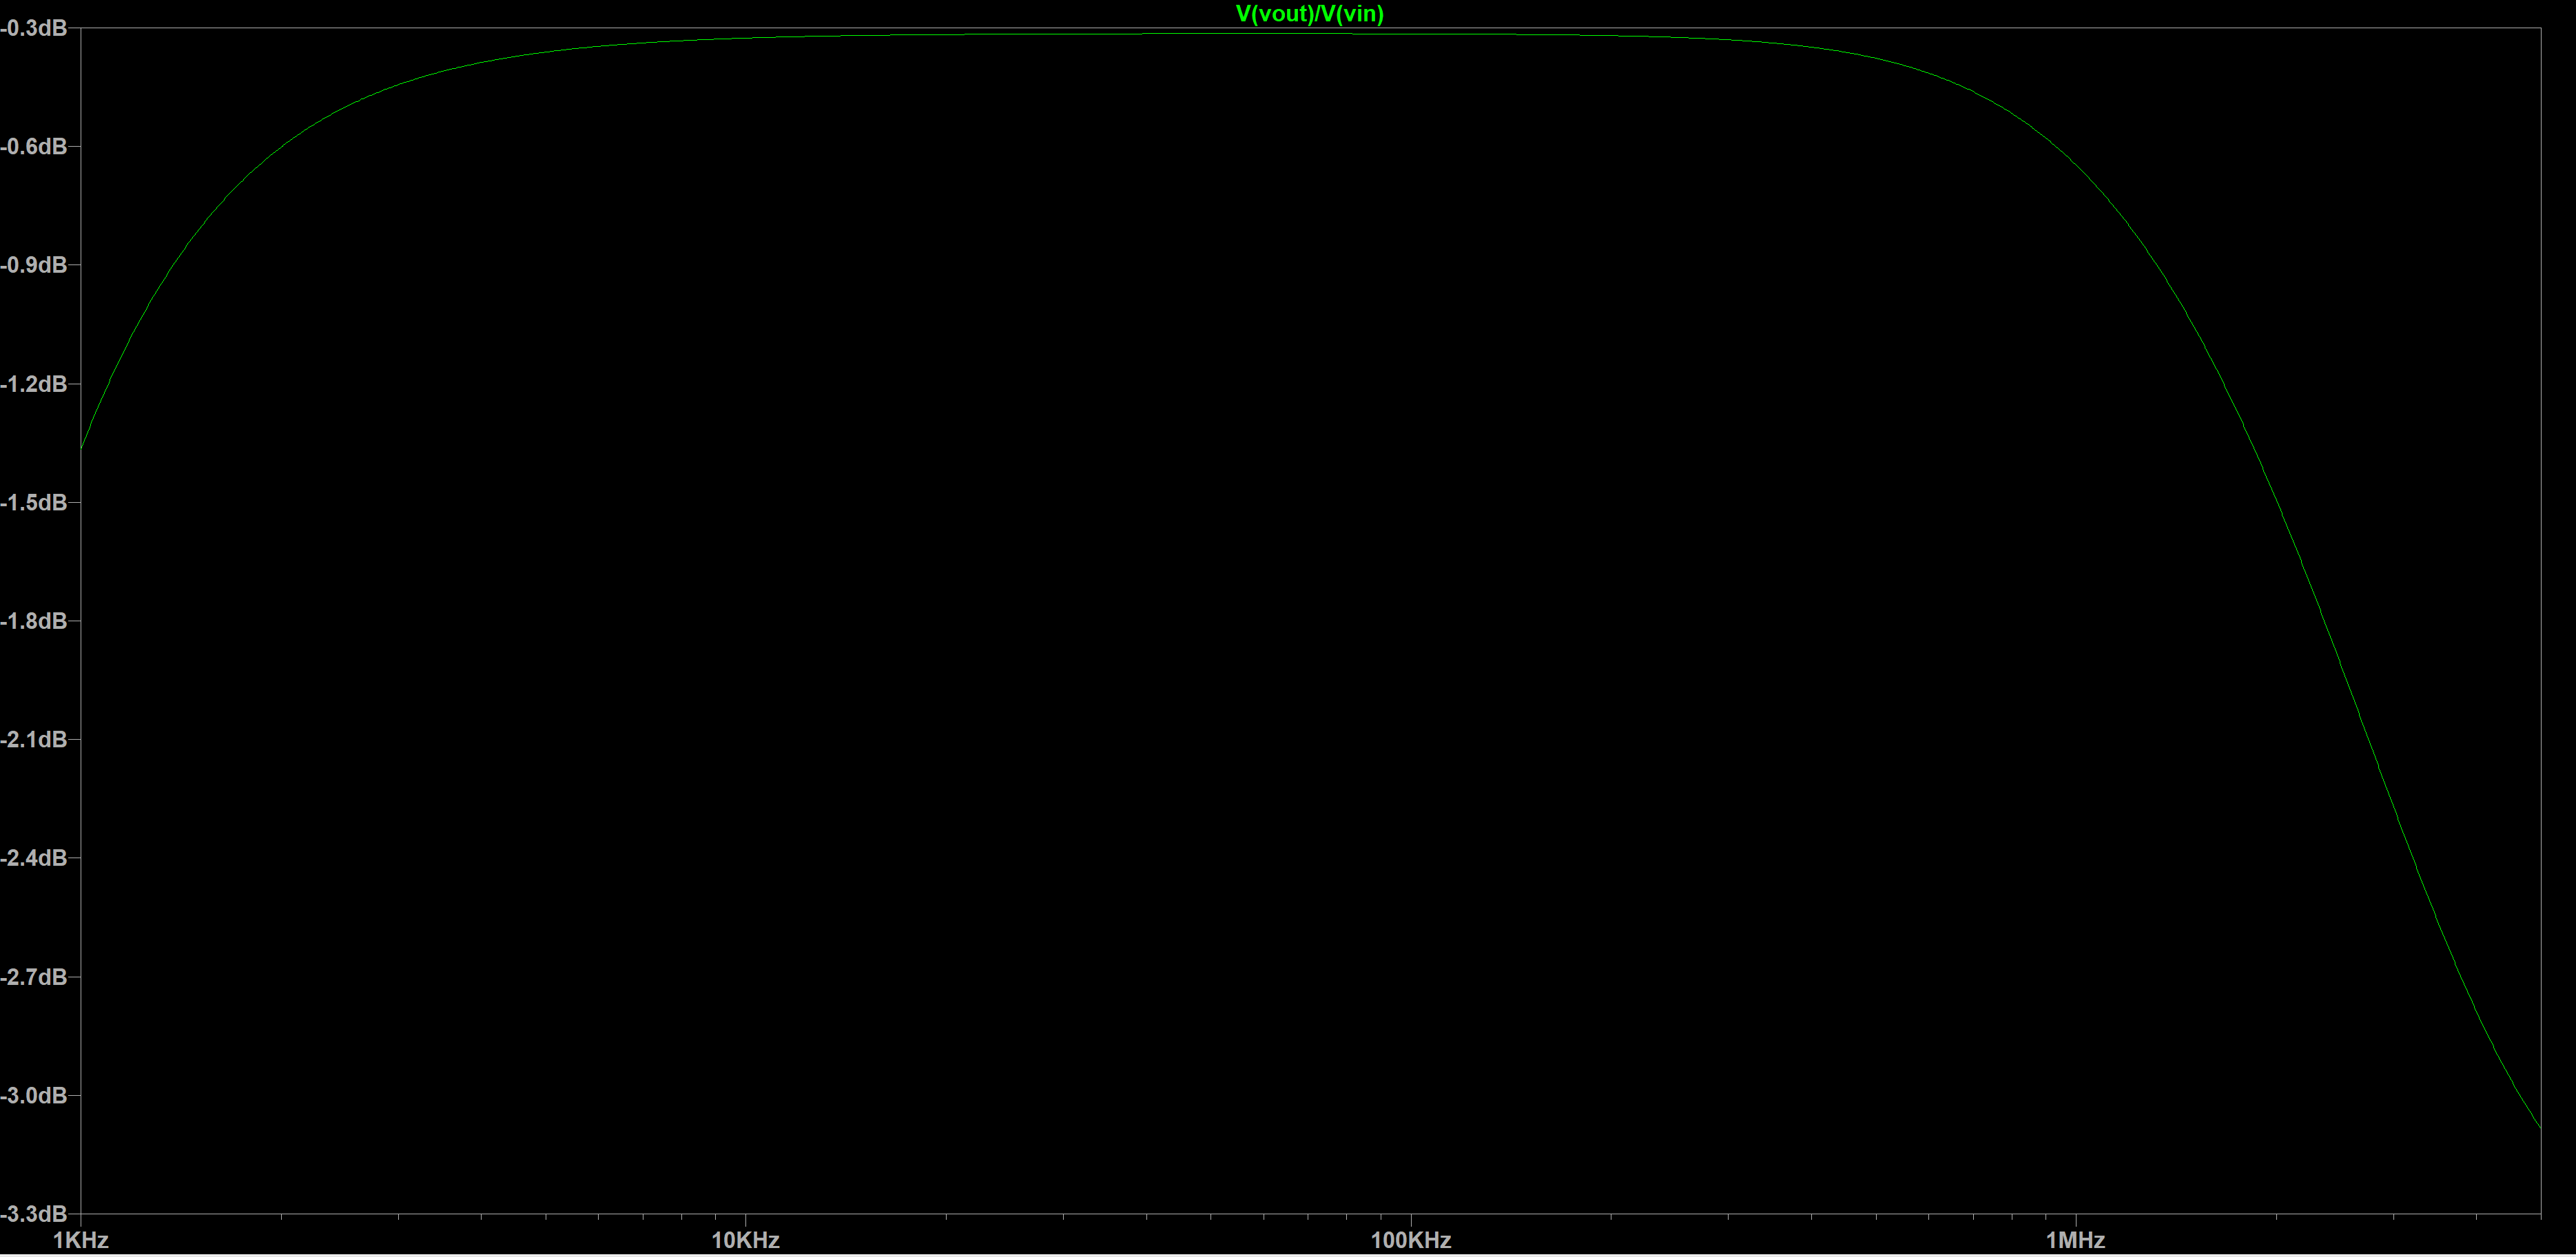
\includegraphics[width=1.0\textwidth]{315.PNG}
    \caption{Buffer Stage Schematic}
\end{figure}

Note that $R_{ee1}$ and $R_{ee2}$ heats sinks are added to prefer thermal runaway.
    

\subsection*{4.1.3 Determine the input and output resistances of the circuit.}

$R_{in} = \beta^2 (R_{EE} + r_e) = 100 * 100 * (10000 + 100) = 101M \Omega$ \\

$R_{out} = ( r_{o3} || r_{e3} + R_{EE} ) = r_{e3} + R_{EE} = 100 \Omega + 10k \Omega$

\subsection*{4.1.4 Plot the time domain output of the circuit to an input which is comparable to the maximum expected differential amplifier output.}

In the first lab, a simulation was already created for the output hence the input to the buffer stage will be the same plot.

\begin{figure}[H]
\centering
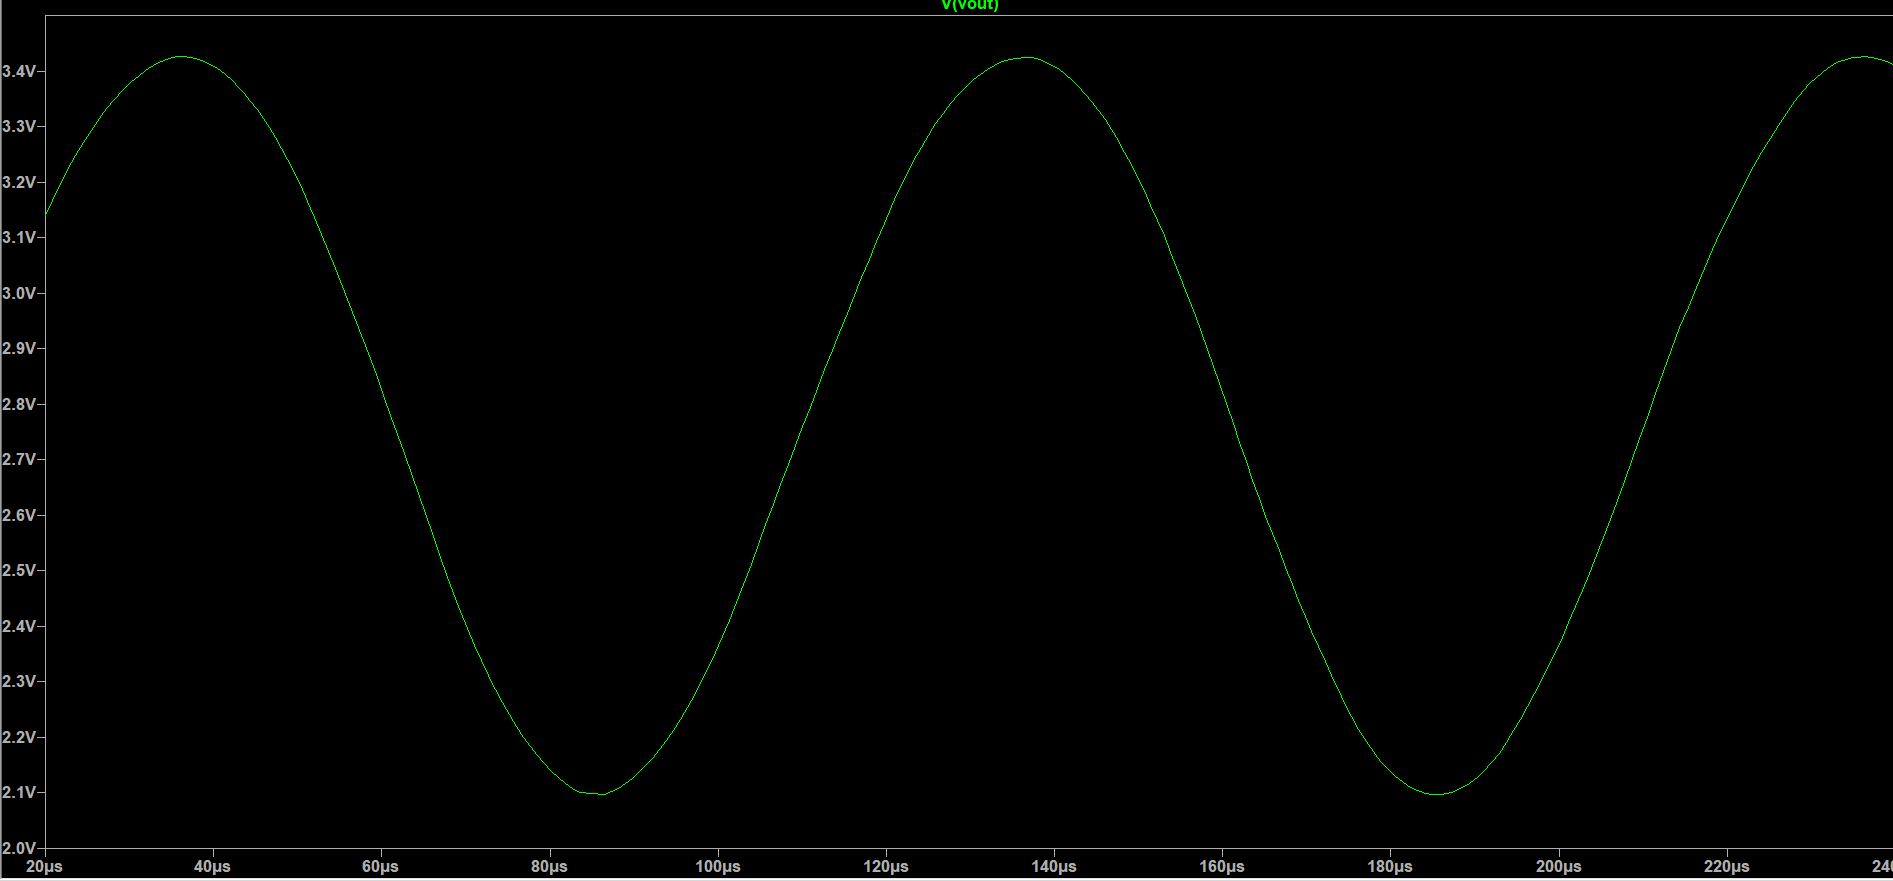
\includegraphics[width=1.0\textwidth]{414.png}
\caption{Input of buffer circuit}
\end{figure}

\subsection*{4.1.5 Plot the frequency response of the circuit. Ensure that the parasitic capacitors are accounted for.}

\begin{figure}[H]
    \centering
    \includegraphics[width=1.0\textwidth]{454.png}
    \caption{Frequency Response}
\end{figure}

\subsection*{4.1.6 Plot the voltage transfer curve of the circuit. Document the maximal output and input ranges.}

\begin{figure}[H]
    \centering
    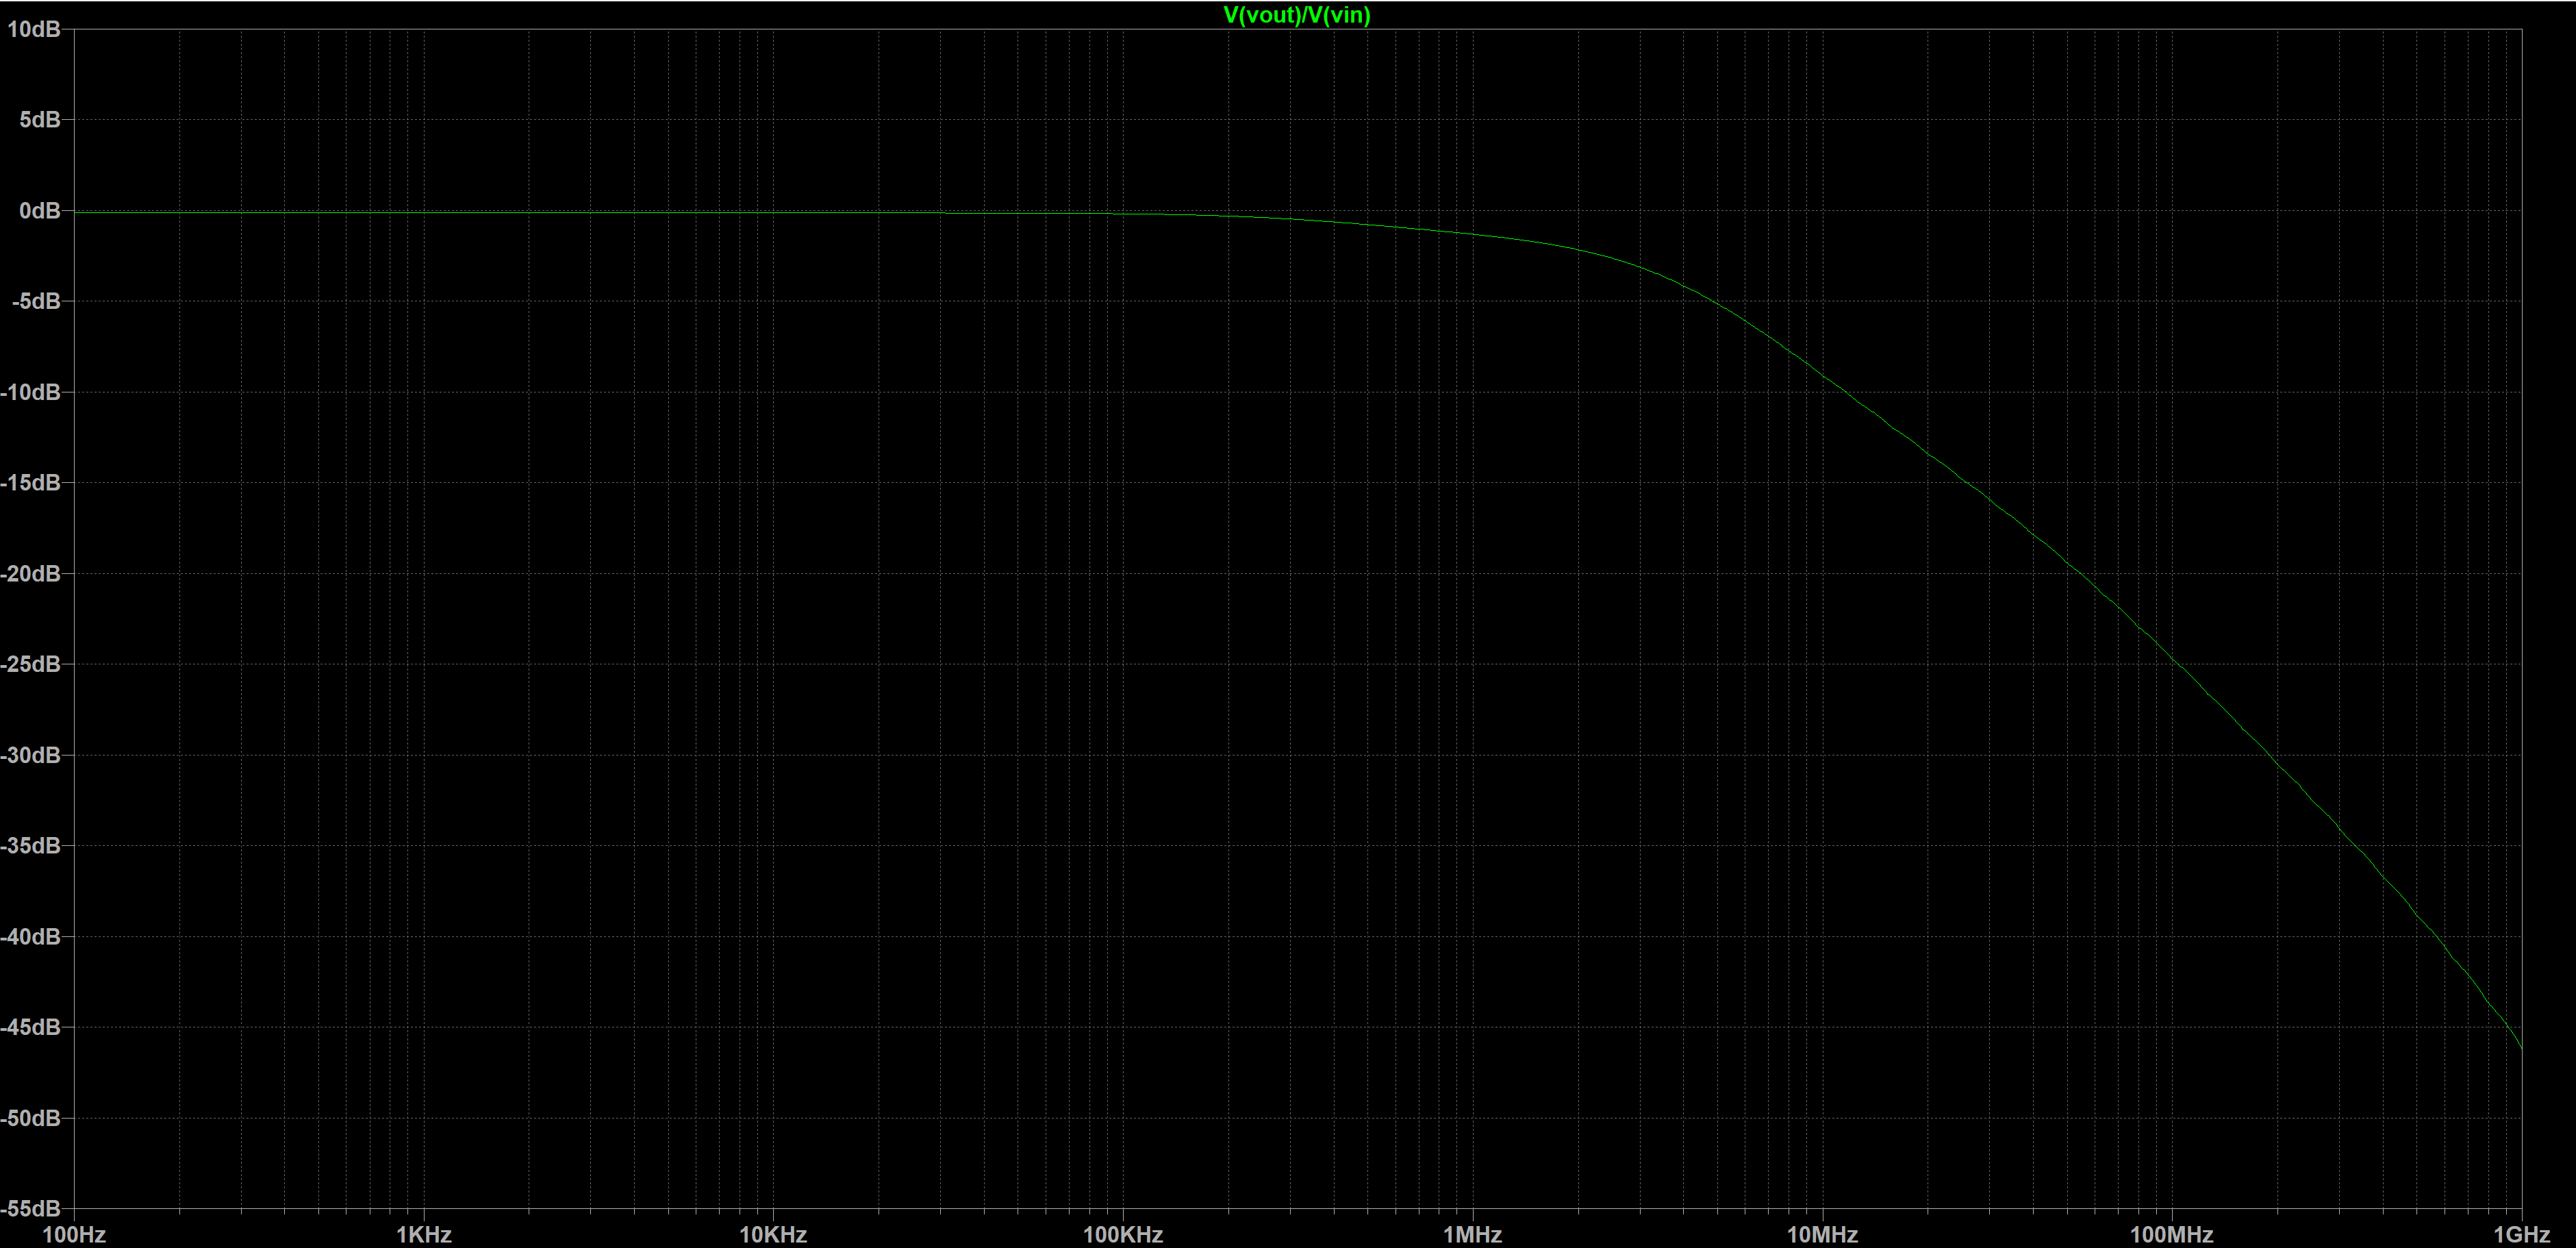
\includegraphics[width=1.0\textwidth]{415.png}
    \caption{Voltage Transfer Curve}
\end{figure}

As shown in the plot, the maximum output voltage 
ranges from approximately -5 to 4.1V with a corresponding
maximum input range from -3.9 V to 4.1 V.

\subsection*{3.1.7 Comment of the advantages and disadvantages of your design.}

The advantages of the design are: 
\begin{itemize}
    \item It has a large bandwidth.
    \item It has a unity gain.
    \item It is simple to implement.
\end{itemize} \\

The disadvantages of the design are: 
\begin{itemize}
    \item It consumes a lot of power because it is still consuming current without any input running through.
    \item $R_{EE}$ has to be limited to a certain number since too high a resistance will cause unwanted loading at the output.
\end{itemize}

\end{document}